\section{conclusion:}

In Figure \ref{fig:test_model} we can see the scores of the \textbf{VILMA} tests, for various models, where the letters \textbf{P} represent the main test and the \textbf{T} represents the \textbf{Proficiency test}.

These are ordered as follows, the first 2 are the \textbf{simple LM}, the next 2 are the \textbf{ILM}, and the rest are the \textbf{VidLM}.

\textbf{Observations from figure 2:}

So we can notice that the best scores are for the Image Language Model (ILM), the VidLMs have score aceptable, and as it was waiting, the LM are the ones with the lowest score, because they do not have images to validate some tests.

We can also noted that simple LMs have good scores in proficiency tests, since these do not imply a strong spatio-temporal relations.
\begin{figure}[h]
    \centering
    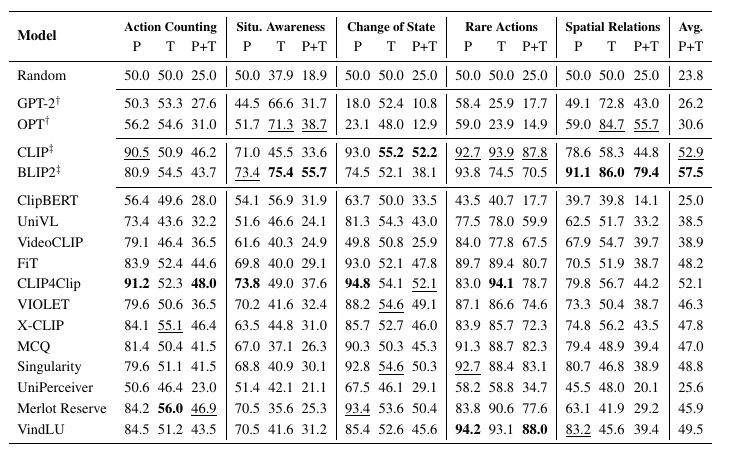
\includegraphics[width=0.25\textwidth]{test_model}
    \caption{Score of the models where the VILMA test was carried out}
    \label{fig:test_model}
\end{figure}

Therefore, I can conclud that VILMA is more focused on VidLM that has spatio-temporal relations for videos, and is also very good for ILM, since the frames of a video are images and VILMA uses a constant frequency of frames to carry out their tests, which allows us to have images that represent periods of frames, and with this method a video could be considered as a set of images but with a space-time relations.
